
% !TEX encoding = UTF-8 Unicode 
% !TEX root = on_gates.tex

\clearpage


\clearpage
\section{Introduction: Gates, states, and circuits}


\begin{quote}
\emph{We shouldn't be asking `where do quantum speedups come from?' we should say `all computers are quantum, [...]' and ask `where do classical slowdowns come from?'} --- Charlie Bennett~\cite{???}
\end{quote}


\begin{quote}
\emph{It appears that very rapid progress is now being made on the fundamentals of quantum computing. It is well to keep in mind, though, that many basic issues of the realization of quantum computers remain unsolved or very difficult.} --- David P. DiVincenzo ~\cite{DiVincenzo1995a}
\end{quote}

%\subsection{???} 
%
%
%\[
%\text{\adjustbox{scale=0.75}{ \documentclass[border=5pt]{standalone}
     \usepackage[svgnames]{xcolor}
   
    \usepackage{tikz}
    \usetikzlibrary{matrix,decorations.pathreplacing, calc, positioning,fit}
    \usepackage{amsmath}
    \usepackage{mathtools}
 
    \begin{document}

    
   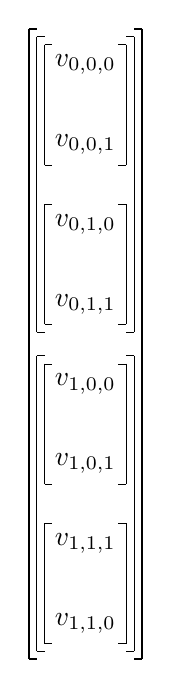
\begin{tikzpicture}[>=stealth,thick,baseline]
    \matrix [matrix of math nodes, row sep=1.5em, column sep=1.5em,](A){ 
    v_{0,0,0} \\
    v_{0,0,1} \\
    v_{0,1,0} \\
	v_{0,1,1} \\
	v_{1,0,0} \\
	v_{1,0,1} \\
	v_{1,1,1} \\ 
    v_{1,1,0} \\
    };
    

%	\draw (A-1-1.north west){}+(-0.1,+0.1) -- (A-1-1){}+(2,0);

	\draw[]  ($(A-1-1.north west) + (-0.2,+0.2)$) -- ($(A-8-1.south west) + (-0.2,-0.2)$);
	\draw[]  ($(A-1-1.north west) + (-0.2,+0.2)$) -- ++(0.1,0);
	\draw[]  ($(A-8-1.south west) + (-0.2,-0.2)$) -- ++(0.1,0); 	

	\draw[]  ($(A-1-1.north east) + (+0.2,+0.2)$) -- ($(A-8-1.south east) + (+0.2,-0.2)$);
	\draw[]  ($(A-1-1.north east) + (+0.2,+0.2)$) -- ++(-0.1,0);
	\draw[]  ($(A-8-1.south east) + (+0.2,-0.2)$) -- ++(-0.1,0); 	


	\draw[thin]  ($(A-1-1.north west) + (-0.1,+0.1)$) -- ($(A-4-1.south west) + (-0.1,-0.1)$);
	\draw[thin]  ($(A-1-1.north west) + (-0.1,+0.1)$) -- ++(0.1,0);
	\draw[thin]  ($(A-4-1.south west) + (-0.1,-0.1)$) -- ++(0.1,0);

	\draw[thin]  ($(A-5-1.north west) + (-0.1,+0.1)$) -- ($(A-8-1.south west) + (-0.1,-0.1)$);
	\draw[thin]  ($(A-5-1.north west) + (-0.1,+0.1)$) -- ++(0.1,0);
	\draw[thin]  ($(A-8-1.south west) + (-0.1,-0.1)$) -- ++(0.1,0);


	\draw[thin]  ($(A-1-1.north east) + (+0.1,+0.1)$) -- ($(A-4-1.south east) + (+0.1,-0.1)$);
	\draw[thin]  ($(A-1-1.north east) + (+0.1,+0.1)$) -- ++(-0.1,0);
	\draw[thin]  ($(A-4-1.south east) + (+0.1,-0.1)$) -- ++(-0.1,0);

	\draw[thin]  ($(A-5-1.north east) + (+0.1,+0.1)$) -- ($(A-8-1.south east) + (+0.1,-0.1)$);
	\draw[thin]  ($(A-5-1.north east) + (+0.1,+0.1)$) -- ++(-0.1,0);
	\draw[thin]  ($(A-8-1.south east) + (+0.1,-0.1)$) -- ++(-0.1,0);




	\draw[ultra thin]  (A-1-1.north west) -- ++(0.1,0);
	\draw[ultra thin]  (A-1-1.north west) -- 
	                   (A-2-1.south west);
	\draw[ultra thin]  (A-2-1.south west) -- ++(0.1,0);	
	
	\draw[ultra thin]  (A-1-1.north east) -- ++(-0.1,0);
	\draw[ultra thin]  (A-1-1.north east) -- 
	                   (A-2-1.south east);
	\draw[ultra thin]  (A-2-1.south east) -- ++(-0.1,0);	
	
	\draw[ultra thin]  (A-3-1.north west) -- ++(0.1,0);
	\draw[ultra thin]  (A-3-1.north west) -- 
	                   (A-4-1.south west);
	\draw[ultra thin]  (A-4-1.south west) -- ++(0.1,0);	
	
	\draw[ultra thin]  (A-3-1.north east) -- ++(-0.1,0);
	\draw[ultra thin]  (A-3-1.north east) -- 
	                   (A-4-1.south east);
	\draw[ultra thin]  (A-4-1.south east) -- ++(-0.1,0);	
	
	\draw[ultra thin]  (A-5-1.north west) -- ++(0.1,0);
	\draw[ultra thin]  (A-5-1.north west) -- 
	                   (A-6-1.south west);
	\draw[ultra thin]  (A-6-1.south west) -- ++(0.1,0);	
	
	\draw[ultra thin]  (A-5-1.north east) -- ++(-0.1,0);
	\draw[ultra thin]  (A-5-1.north east) -- 
	                   (A-6-1.south east);
	\draw[ultra thin]  (A-6-1.south east) -- ++(-0.1,0);	
	
	\draw[ultra thin]  (A-7-1.north west) -- ++(0.1,0);
	\draw[ultra thin]  (A-7-1.north west) -- 
	                   (A-8-1.south west);
	\draw[ultra thin]  (A-8-1.south west) -- ++(0.1,0);	
	
	\draw[ultra thin]  (A-7-1.north east) -- ++(-0.1,0);
	\draw[ultra thin]  (A-7-1.north east) -- 
	                   (A-8-1.south east);
	\draw[ultra thin]  (A-8-1.south east) -- ++(-0.1,0);	


    \end{tikzpicture}

    
    
\end{document}
    
    
    }} 
%=
%\text{\adjustbox{scale=0.75}{ \documentclass[border=5pt]{standalone}
     \usepackage[svgnames]{xcolor}
   
    \usepackage{tikz}
    \usetikzlibrary{matrix,decorations.pathreplacing, calc, positioning,fit}
    \usepackage{amsmath}
    \usepackage{mathtools}
 
    \begin{document}

    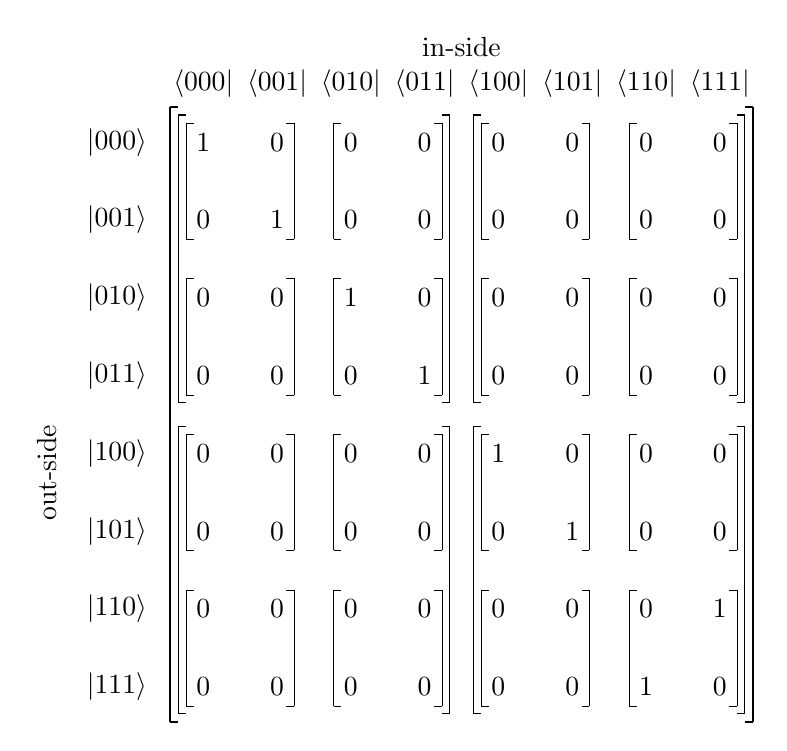
\begin{tikzpicture}[>=stealth,thick,baseline]
    \matrix [matrix of math nodes, row sep=1.5em, column sep=1.5em,](A){ 
    1&0&0&0&0&0&0&0 \\
    0&1&0&0&0&0&0&0 \\
    0&0&1&0&0&0&0&0 \\
	0&0&0&1&0&0&0&0 \\
	0&0&0&0&1&0&0&0 \\
	0&0&0&0&0&1&0&0 \\
	0&0&0&0&0&0&0&1 \\
    0&0&0&0&0&0&1&0 \\
    };

	\draw[]  ($(A-1-1.north west) + (-0.2,+0.2)$) -- ($(A-8-1.south west) + (-0.2,-0.2)$);
	\draw[]  ($(A-1-1.north west) + (-0.2,+0.2)$) -- ++(0.1,0);
	\draw[]  ($(A-8-1.south west) + (-0.2,-0.2)$) -- ++(0.1,0); 	

	\draw[]  ($(A-1-8.north east) + (+0.2,+0.2)$) -- ($(A-8-8.south east) + (+0.2,-0.2)$);
	\draw[]  ($(A-1-8.north east) + (+0.2,+0.2)$) -- ++(-0.1,0);
	\draw[]  ($(A-8-8.south east) + (+0.2,-0.2)$) -- ++(-0.1,0); 	


	\draw[thin]  ($(A-1-1.north west) + (-0.1,+0.1)$) -- ($(A-4-1.south west) + (-0.1,-0.1)$);
	\draw[thin]  ($(A-1-1.north west) + (-0.1,+0.1)$) -- ++(0.1,0);
	\draw[thin]  ($(A-4-1.south west) + (-0.1,-0.1)$) -- ++(0.1,0);

	\draw[thin]  ($(A-5-1.north west) + (-0.1,+0.1)$) -- ($(A-8-1.south west) + (-0.1,-0.1)$);
	\draw[thin]  ($(A-5-1.north west) + (-0.1,+0.1)$) -- ++(0.1,0);
	\draw[thin]  ($(A-8-1.south west) + (-0.1,-0.1)$) -- ++(0.1,0);

	\draw[thin]  ($(A-1-5.north west) + (-0.1,+0.1)$) -- ($(A-4-5.south west) + (-0.1,-0.1)$);
	\draw[thin]  ($(A-1-5.north west) + (-0.1,+0.1)$) -- ++(0.1,0);
	\draw[thin]  ($(A-4-5.south west) + (-0.1,-0.1)$) -- ++(0.1,0);

	\draw[thin]  ($(A-5-5.north west) + (-0.1,+0.1)$) -- ($(A-8-5.south west) + (-0.1,-0.1)$);
	\draw[thin]  ($(A-5-5.north west) + (-0.1,+0.1)$) -- ++(0.1,0);
	\draw[thin]  ($(A-8-5.south west) + (-0.1,-0.1)$) -- ++(0.1,0);


	\draw[thin]  ($(A-1-4.north east) + (+0.1,+0.1)$) -- ($(A-4-4.south east) + (+0.1,-0.1)$);
	\draw[thin]  ($(A-1-4.north east) + (+0.1,+0.1)$) -- ++(-0.1,0);
	\draw[thin]  ($(A-4-4.south east) + (+0.1,-0.1)$) -- ++(-0.1,0);

	\draw[thin]  ($(A-5-4.north east) + (+0.1,+0.1)$) -- ($(A-8-4.south east) + (+0.1,-0.1)$);
	\draw[thin]  ($(A-5-4.north east) + (+0.1,+0.1)$) -- ++(-0.1,0);
	\draw[thin]  ($(A-8-4.south east) + (+0.1,-0.1)$) -- ++(-0.1,0);


	\draw[thin]  ($(A-1-8.north east) + (+0.1,+0.1)$) -- ($(A-4-8.south east) + (+0.1,-0.1)$);
	\draw[thin]  ($(A-1-8.north east) + (+0.1,+0.1)$) -- ++(-0.1,0);
	\draw[thin]  ($(A-4-8.south east) + (+0.1,-0.1)$) -- ++(-0.1,0);

	\draw[thin]  ($(A-5-8.north east) + (+0.1,+0.1)$) -- ($(A-8-8.south east) + (+0.1,-0.1)$);
	\draw[thin]  ($(A-5-8.north east) + (+0.1,+0.1)$) -- ++(-0.1,0);
	\draw[thin]  ($(A-8-8.south east) + (+0.1,-0.1)$) -- ++(-0.1,0);


	\draw[ultra thin]  (A-1-1.north west) -- ++(0.1,0);
	\draw[ultra thin]  (A-1-1.north west) -- 
	                   (A-2-1.south west);
	\draw[ultra thin]  (A-2-1.south west) -- ++(0.1,0);	
	
	\draw[ultra thin]  (A-1-2.north east) -- ++(-0.1,0);
	\draw[ultra thin]  (A-1-2.north east) -- 
	                   (A-2-2.south east);
	\draw[ultra thin]  (A-2-2.south east) -- ++(-0.1,0);	
	
	\draw[ultra thin]  (A-3-1.north west) -- ++(0.1,0);
	\draw[ultra thin]  (A-3-1.north west) -- 
	                   (A-4-1.south west);
	\draw[ultra thin]  (A-4-1.south west) -- ++(0.1,0);	
	
	\draw[ultra thin]  (A-3-2.north east) -- ++(-0.1,0);
	\draw[ultra thin]  (A-3-2.north east) -- 
	                   (A-4-2.south east);
	\draw[ultra thin]  (A-4-2.south east) -- ++(-0.1,0);	
	
	\draw[ultra thin]  (A-5-1.north west) -- ++(0.1,0);
	\draw[ultra thin]  (A-5-1.north west) -- 
	                   (A-6-1.south west);
	\draw[ultra thin]  (A-6-1.south west) -- ++(0.1,0);	
	
	\draw[ultra thin]  (A-5-2.north east) -- ++(-0.1,0);
	\draw[ultra thin]  (A-5-2.north east) -- 
	                   (A-6-2.south east);
	\draw[ultra thin]  (A-6-2.south east) -- ++(-0.1,0);	
	
	\draw[ultra thin]  (A-7-1.north west) -- ++(0.1,0);
	\draw[ultra thin]  (A-7-1.north west) -- 
	                   (A-8-1.south west);
	\draw[ultra thin]  (A-8-1.south west) -- ++(0.1,0);	
	
	\draw[ultra thin]  (A-7-2.north east) -- ++(-0.1,0);
	\draw[ultra thin]  (A-7-2.north east) -- 
	                   (A-8-2.south east);
	\draw[ultra thin]  (A-8-2.south east) -- ++(-0.1,0);	


	\draw[ultra thin]  (A-1-3.north west) -- ++(0.1,0);
	\draw[ultra thin]  (A-1-3.north west) -- 
	                   (A-2-3.south west);
	\draw[ultra thin]  (A-2-3.south west) -- ++(0.1,0);	
	
	\draw[ultra thin]  (A-1-4.north east) -- ++(-0.1,0);
	\draw[ultra thin]  (A-1-4.north east) -- 
	                   (A-2-4.south east);
	\draw[ultra thin]  (A-2-4.south east) -- ++(-0.1,0);	
	
	\draw[ultra thin]  (A-3-3.north west) -- ++(0.1,0);
	\draw[ultra thin]  (A-3-3.north west) -- 
	                   (A-4-3.south west);
	\draw[ultra thin]  (A-4-3.south west) -- ++(0.1,0);	
	
	\draw[ultra thin]  (A-3-4.north east) -- ++(-0.1,0);
	\draw[ultra thin]  (A-3-4.north east) -- 
	                   (A-4-4.south east);
	\draw[ultra thin]  (A-4-4.south east) -- ++(-0.1,0);	
	
	\draw[ultra thin]  (A-5-3.north west) -- ++(0.1,0);
	\draw[ultra thin]  (A-5-3.north west) -- 
	                   (A-6-3.south west);
	\draw[ultra thin]  (A-6-3.south west) -- ++(0.1,0);	
	
	\draw[ultra thin]  (A-5-4.north east) -- ++(-0.1,0);
	\draw[ultra thin]  (A-5-4.north east) -- 
	                   (A-6-4.south east);
	\draw[ultra thin]  (A-6-4.south east) -- ++(-0.1,0);	
	
	\draw[ultra thin]  (A-7-3.north west) -- ++(0.1,0);
	\draw[ultra thin]  (A-7-3.north west) -- 
	                   (A-8-3.south west);
	\draw[ultra thin]  (A-8-3.south west) -- ++(0.1,0);	
	
	\draw[ultra thin]  (A-7-4.north east) -- ++(-0.1,0);
	\draw[ultra thin]  (A-7-4.north east) -- 
	                   (A-8-4.south east);
	\draw[ultra thin]  (A-8-4.south east) -- ++(-0.1,0);	
	

	\draw[ultra thin]  (A-1-3.north west) -- ++(0.1,0);
	\draw[ultra thin]  (A-1-3.north west) -- 
	                   (A-2-3.south west);
	\draw[ultra thin]  (A-2-3.south west) -- ++(0.1,0);	
	
	\draw[ultra thin]  (A-1-4.north east) -- ++(-0.1,0);
	\draw[ultra thin]  (A-1-4.north east) -- 
	                   (A-2-4.south east);
	\draw[ultra thin]  (A-2-4.south east) -- ++(-0.1,0);	
	
	\draw[ultra thin]  (A-3-3.north west) -- ++(0.1,0);
	\draw[ultra thin]  (A-3-3.north west) -- 
	                   (A-4-3.south west);
	\draw[ultra thin]  (A-4-3.south west) -- ++(0.1,0);	
	
	\draw[ultra thin]  (A-3-4.north east) -- ++(-0.1,0);
	\draw[ultra thin]  (A-3-4.north east) -- 
	                   (A-4-4.south east);
	\draw[ultra thin]  (A-4-4.south east) -- ++(-0.1,0);	
	
	\draw[ultra thin]  (A-5-3.north west) -- ++(0.1,0);
	\draw[ultra thin]  (A-5-3.north west) -- 
	                   (A-6-3.south west);
	\draw[ultra thin]  (A-6-3.south west) -- ++(0.1,0);	
	
	\draw[ultra thin]  (A-5-4.north east) -- ++(-0.1,0);
	\draw[ultra thin]  (A-5-4.north east) -- 
	                   (A-6-4.south east);
	\draw[ultra thin]  (A-6-4.south east) -- ++(-0.1,0);	
	
	\draw[ultra thin]  (A-7-3.north west) -- ++(0.1,0);
	\draw[ultra thin]  (A-7-3.north west) -- 
	                   (A-8-3.south west);
	\draw[ultra thin]  (A-8-3.south west) -- ++(0.1,0);	
	
	\draw[ultra thin]  (A-7-4.north east) -- ++(-0.1,0);
	\draw[ultra thin]  (A-7-4.north east) -- 
	                   (A-8-4.south east);
	\draw[ultra thin]  (A-8-4.south east) -- ++(-0.1,0);	
	
	

	\draw[ultra thin]  (A-1-5.north west) -- ++(0.1,0);
	\draw[ultra thin]  (A-1-5.north west) -- 
	                   (A-2-5.south west);
	\draw[ultra thin]  (A-2-5.south west) -- ++(0.1,0);	
	
	\draw[ultra thin]  (A-1-6.north east) -- ++(-0.1,0);
	\draw[ultra thin]  (A-1-6.north east) -- 
	                   (A-2-6.south east);
	\draw[ultra thin]  (A-2-6.south east) -- ++(-0.1,0);	
	
	\draw[ultra thin]  (A-3-5.north west) -- ++(0.1,0);
	\draw[ultra thin]  (A-3-5.north west) -- 
	                   (A-4-5.south west);
	\draw[ultra thin]  (A-4-5.south west) -- ++(0.1,0);	
	
	\draw[ultra thin]  (A-3-6.north east) -- ++(-0.1,0);
	\draw[ultra thin]  (A-3-6.north east) -- 
	                   (A-4-6.south east);
	\draw[ultra thin]  (A-4-6.south east) -- ++(-0.1,0);	
	
	\draw[ultra thin]  (A-5-5.north west) -- ++(0.1,0);
	\draw[ultra thin]  (A-5-5.north west) -- 
	                   (A-6-5.south west);
	\draw[ultra thin]  (A-6-5.south west) -- ++(0.1,0);	
	
	\draw[ultra thin]  (A-5-6.north east) -- ++(-0.1,0);
	\draw[ultra thin]  (A-5-6.north east) -- 
	                   (A-6-6.south east);
	\draw[ultra thin]  (A-6-6.south east) -- ++(-0.1,0);	
	
	\draw[ultra thin]  (A-7-5.north west) -- ++(0.1,0);
	\draw[ultra thin]  (A-7-5.north west) -- 
	                   (A-8-5.south west);
	\draw[ultra thin]  (A-8-5.south west) -- ++(0.1,0);	
	
	\draw[ultra thin]  (A-7-6.north east) -- ++(-0.1,0);
	\draw[ultra thin]  (A-7-6.north east) -- 
	                   (A-8-6.south east);
	\draw[ultra thin]  (A-8-6.south east) -- ++(-0.1,0);	
		
	
	
	
	
	\draw[ultra thin]  (A-1-7.north west) -- ++(0.1,0);
	\draw[ultra thin]  (A-1-7.north west) -- 
	                   (A-2-7.south west);
	\draw[ultra thin]  (A-2-7.south west) -- ++(0.1,0);	
	
	\draw[ultra thin]  (A-1-8.north east) -- ++(-0.1,0);
	\draw[ultra thin]  (A-1-8.north east) -- 
	                   (A-2-8.south east);
	\draw[ultra thin]  (A-2-8.south east) -- ++(-0.1,0);	
	
	\draw[ultra thin]  (A-3-7.north west) -- ++(0.1,0);
	\draw[ultra thin]  (A-3-7.north west) -- 
	                   (A-4-7.south west);
	\draw[ultra thin]  (A-4-7.south west) -- ++(0.1,0);	
	
	\draw[ultra thin]  (A-3-8.north east) -- ++(-0.1,0);
	\draw[ultra thin]  (A-3-8.north east) -- 
	                   (A-4-8.south east);
	\draw[ultra thin]  (A-4-8.south east) -- ++(-0.1,0);	
	
	\draw[ultra thin]  (A-5-7.north west) -- ++(0.1,0);
	\draw[ultra thin]  (A-5-7.north west) -- 
	                   (A-6-7.south west);
	\draw[ultra thin]  (A-6-7.south west) -- ++(0.1,0);	
	
	\draw[ultra thin]  (A-5-8.north east) -- ++(-0.1,0);
	\draw[ultra thin]  (A-5-8.north east) -- 
	                   (A-6-8.south east);
	\draw[ultra thin]  (A-6-8.south east) -- ++(-0.1,0);	
	
	\draw[ultra thin]  (A-7-7.north west) -- ++(0.1,0);
	\draw[ultra thin]  (A-7-7.north west) -- 
	                   (A-8-7.south west);
	\draw[ultra thin]  (A-8-7.south west) -- ++(0.1,0);	
	
	\draw[ultra thin]  (A-7-8.north east) -- ++(-0.1,0);
	\draw[ultra thin]  (A-7-8.north east) -- 
	                   (A-8-8.south east);
	\draw[ultra thin]  (A-8-8.south east) -- ++(-0.1,0);	
	
	
   \node[
     fit=(A-1-4)(A-1-5),
     inner xsep=5pt,inner ysep=20pt,
     label=above: in-side   
     ](K01) {};

   \node[
     fit=(A-4-1)(A-5-1),
     inner xsep=50pt,inner ysep=-5pt,
     label={[rotate=90]left:out-side}
     ](K01) {};




   \node[
     fit=(A-1-1)(A-1-1),
     inner xsep=5pt,inner ysep=5pt,
     label=above: $\langle 000|$
    ](K00) {};

   \node[
     fit=(A-1-2)(A-1-2),
     inner xsep=5pt,inner ysep=5pt,
     label=above: $\langle 001|$
    ](K01) {};


   \node[
     fit=(A-1-3)(A-1-3),
     inner xsep=5pt,inner ysep=5pt,
     label=above: $\langle 010|$
    ](K10) {};

   \node[
     fit=(A-1-4)(A-1-4),
     inner xsep=5pt,inner ysep=5pt,
     label=above: $\langle 011|$
    ](K10) {};


   \node[
     fit=(A-1-5)(A-1-5),
     inner xsep=5pt,inner ysep=5pt,
     label=above: $\langle 100|$
    ](K00) {};

   \node[
     fit=(A-1-6)(A-1-6),
     inner xsep=5pt,inner ysep=5pt,
     label=above: $\langle 101|$
    ](K01) {};

   \node[
     fit=(A-1-7)(A-1-7),
     inner xsep=5pt,inner ysep=5pt,
     label=above: $\langle 110|$
    ](K10) {};
   \node[
     fit=(A-1-8)(A-1-8),
     inner xsep=5pt,inner ysep=5pt,
     label=above: $\langle 111|$
    ](K11) {};


   \node[
     fit=(A-1-1)(A-1-1),
     inner xsep=10pt,inner ysep=5pt,
     label=left: $|000\rangle$
    ](K00) {};

   \node[
     fit=(A-2-1)(A-2-1),
     inner xsep=10pt,inner ysep=5pt,
     label=left: $|001\rangle$
    ](K01) {};


   \node[
     fit=(A-3-1)(A-3-1),
     inner xsep=10pt,inner ysep=5pt,
     label=left: $|010\rangle$
    ](K10) {};


   \node[
     fit=(A-4-1)(A-4-1),
     inner xsep=10pt,inner ysep=5pt,
     label=left: $|011\rangle$
    ](K11) {};


   \node[
     fit=(A-5-1)(A-5-1),
     inner xsep=10pt,inner ysep=5pt,
     label=left: $|100\rangle$
    ](K00) {};

   \node[
     fit=(A-6-1)(A-6-1),
     inner xsep=10pt,inner ysep=5pt,
     label=left: $|101\rangle$
    ](K01) {};


   \node[
     fit=(A-7-1)(A-7-1),
     inner xsep=10pt,inner ysep=5pt,
     label=left: $|110\rangle$
    ](K10) {};


   \node[
     fit=(A-8-1)(A-8-1),
     inner xsep=10pt,inner ysep=5pt,
     label=left: $|111\rangle$
    ](K11) {};


    \end{tikzpicture}

\end{document}
    
    
    }}
%\bullet
%\text{\adjustbox{scale=0.75}{ \documentclass[border=5pt]{standalone}
     \usepackage[svgnames]{xcolor}
   
    \usepackage{tikz}
    \usetikzlibrary{matrix,decorations.pathreplacing, calc, positioning,fit}
    \usepackage{amsmath}
    \usepackage{mathtools}
 
    \begin{document}

    
   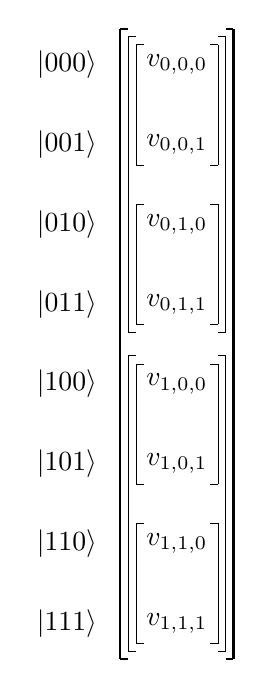
\begin{tikzpicture}[>=stealth,thick,baseline]
    \matrix [matrix of math nodes, row sep=1.5em, column sep=1.5em,](A){ 
    v_{0,0,0} \\
    v_{0,0,1} \\
    v_{0,1,0} \\
	v_{0,1,1} \\
	v_{1,0,0} \\
	v_{1,0,1} \\
	v_{1,1,0} \\ 
    v_{1,1,1} \\
    };
    

%	\draw (A-1-1.north west){}+(-0.1,+0.1) -- (A-1-1){}+(2,0);

	\draw[]  ($(A-1-1.north west) + (-0.2,+0.2)$) -- ($(A-8-1.south west) + (-0.2,-0.2)$);
	\draw[]  ($(A-1-1.north west) + (-0.2,+0.2)$) -- ++(0.1,0);
	\draw[]  ($(A-8-1.south west) + (-0.2,-0.2)$) -- ++(0.1,0); 	

	\draw[]  ($(A-1-1.north east) + (+0.2,+0.2)$) -- ($(A-8-1.south east) + (+0.2,-0.2)$);
	\draw[]  ($(A-1-1.north east) + (+0.2,+0.2)$) -- ++(-0.1,0);
	\draw[]  ($(A-8-1.south east) + (+0.2,-0.2)$) -- ++(-0.1,0); 	


	\draw[thin]  ($(A-1-1.north west) + (-0.1,+0.1)$) -- ($(A-4-1.south west) + (-0.1,-0.1)$);
	\draw[thin]  ($(A-1-1.north west) + (-0.1,+0.1)$) -- ++(0.1,0);
	\draw[thin]  ($(A-4-1.south west) + (-0.1,-0.1)$) -- ++(0.1,0);

	\draw[thin]  ($(A-5-1.north west) + (-0.1,+0.1)$) -- ($(A-8-1.south west) + (-0.1,-0.1)$);
	\draw[thin]  ($(A-5-1.north west) + (-0.1,+0.1)$) -- ++(0.1,0);
	\draw[thin]  ($(A-8-1.south west) + (-0.1,-0.1)$) -- ++(0.1,0);


	\draw[thin]  ($(A-1-1.north east) + (+0.1,+0.1)$) -- ($(A-4-1.south east) + (+0.1,-0.1)$);
	\draw[thin]  ($(A-1-1.north east) + (+0.1,+0.1)$) -- ++(-0.1,0);
	\draw[thin]  ($(A-4-1.south east) + (+0.1,-0.1)$) -- ++(-0.1,0);

	\draw[thin]  ($(A-5-1.north east) + (+0.1,+0.1)$) -- ($(A-8-1.south east) + (+0.1,-0.1)$);
	\draw[thin]  ($(A-5-1.north east) + (+0.1,+0.1)$) -- ++(-0.1,0);
	\draw[thin]  ($(A-8-1.south east) + (+0.1,-0.1)$) -- ++(-0.1,0);




	\draw[ultra thin]  (A-1-1.north west) -- ++(0.1,0);
	\draw[ultra thin]  (A-1-1.north west) -- 
	                   (A-2-1.south west);
	\draw[ultra thin]  (A-2-1.south west) -- ++(0.1,0);	
	
	\draw[ultra thin]  (A-1-1.north east) -- ++(-0.1,0);
	\draw[ultra thin]  (A-1-1.north east) -- 
	                   (A-2-1.south east);
	\draw[ultra thin]  (A-2-1.south east) -- ++(-0.1,0);	
	
	\draw[ultra thin]  (A-3-1.north west) -- ++(0.1,0);
	\draw[ultra thin]  (A-3-1.north west) -- 
	                   (A-4-1.south west);
	\draw[ultra thin]  (A-4-1.south west) -- ++(0.1,0);	
	
	\draw[ultra thin]  (A-3-1.north east) -- ++(-0.1,0);
	\draw[ultra thin]  (A-3-1.north east) -- 
	                   (A-4-1.south east);
	\draw[ultra thin]  (A-4-1.south east) -- ++(-0.1,0);	
	
	\draw[ultra thin]  (A-5-1.north west) -- ++(0.1,0);
	\draw[ultra thin]  (A-5-1.north west) -- 
	                   (A-6-1.south west);
	\draw[ultra thin]  (A-6-1.south west) -- ++(0.1,0);	
	
	\draw[ultra thin]  (A-5-1.north east) -- ++(-0.1,0);
	\draw[ultra thin]  (A-5-1.north east) -- 
	                   (A-6-1.south east);
	\draw[ultra thin]  (A-6-1.south east) -- ++(-0.1,0);	
	
	\draw[ultra thin]  (A-7-1.north west) -- ++(0.1,0);
	\draw[ultra thin]  (A-7-1.north west) -- 
	                   (A-8-1.south west);
	\draw[ultra thin]  (A-8-1.south west) -- ++(0.1,0);	
	
	\draw[ultra thin]  (A-7-1.north east) -- ++(-0.1,0);
	\draw[ultra thin]  (A-7-1.north east) -- 
	                   (A-8-1.south east);
	\draw[ultra thin]  (A-8-1.south east) -- ++(-0.1,0);	


   \node[
     fit=(A-1-1)(A-1-1),
     inner xsep=10pt,inner ysep=5pt,
     label=left: $|000\rangle$
    ](K00) {};

   \node[
     fit=(A-2-1)(A-2-1),
     inner xsep=10pt,inner ysep=5pt,
     label=left: $|001\rangle$
    ](K01) {};


   \node[
     fit=(A-3-1)(A-3-1),
     inner xsep=10pt,inner ysep=5pt,
     label=left: $|010\rangle$
    ](K10) {};


   \node[
     fit=(A-4-1)(A-4-1),
     inner xsep=10pt,inner ysep=5pt,
     label=left: $|011\rangle$
    ](K11) {};


   \node[
     fit=(A-5-1)(A-5-1),
     inner xsep=10pt,inner ysep=5pt,
     label=left: $|100\rangle$
    ](K00) {};

   \node[
     fit=(A-6-1)(A-6-1),
     inner xsep=10pt,inner ysep=5pt,
     label=left: $|101\rangle$
    ](K01) {};


   \node[
     fit=(A-7-1)(A-7-1),
     inner xsep=10pt,inner ysep=5pt,
     label=left: $|110\rangle$
    ](K10) {};


   \node[
     fit=(A-8-1)(A-8-1),
     inner xsep=10pt,inner ysep=5pt,
     label=left: $|111\rangle$
    ](K11) {};

%   \node[
%     fit=(A-6-4)(A-6-4),
%     inner xsep=20pt,inner ysep=20pt,
%     label=below: $j$-ième colonne
%     ](C) {};
%
%    \draw[->](L.east)-- (A-4-4);
%    \draw[->](C.south)-- (A-4-4);

    \end{tikzpicture}

    
    
\end{document}
    
    
    }}
%\]
%%=  \dot  \documentclass[border=5pt]{standalone}
     \usepackage[svgnames]{xcolor}
   
    \usepackage{tikz}
    \usetikzlibrary{matrix,decorations.pathreplacing, calc, positioning,fit}
    \usepackage{amsmath}
    \usepackage{mathtools}
 
    \begin{document}

    
   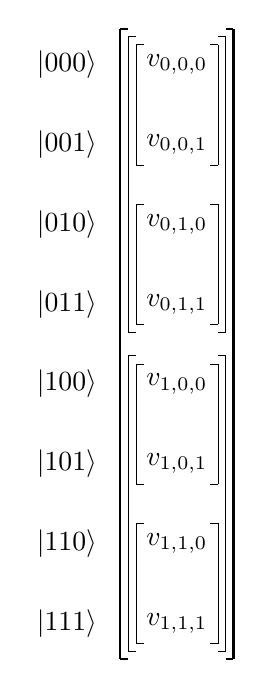
\begin{tikzpicture}[>=stealth,thick,baseline]
    \matrix [matrix of math nodes, row sep=1.5em, column sep=1.5em,](A){ 
    v_{0,0,0} \\
    v_{0,0,1} \\
    v_{0,1,0} \\
	v_{0,1,1} \\
	v_{1,0,0} \\
	v_{1,0,1} \\
	v_{1,1,0} \\ 
    v_{1,1,1} \\
    };
    

%	\draw (A-1-1.north west){}+(-0.1,+0.1) -- (A-1-1){}+(2,0);

	\draw[]  ($(A-1-1.north west) + (-0.2,+0.2)$) -- ($(A-8-1.south west) + (-0.2,-0.2)$);
	\draw[]  ($(A-1-1.north west) + (-0.2,+0.2)$) -- ++(0.1,0);
	\draw[]  ($(A-8-1.south west) + (-0.2,-0.2)$) -- ++(0.1,0); 	

	\draw[]  ($(A-1-1.north east) + (+0.2,+0.2)$) -- ($(A-8-1.south east) + (+0.2,-0.2)$);
	\draw[]  ($(A-1-1.north east) + (+0.2,+0.2)$) -- ++(-0.1,0);
	\draw[]  ($(A-8-1.south east) + (+0.2,-0.2)$) -- ++(-0.1,0); 	


	\draw[thin]  ($(A-1-1.north west) + (-0.1,+0.1)$) -- ($(A-4-1.south west) + (-0.1,-0.1)$);
	\draw[thin]  ($(A-1-1.north west) + (-0.1,+0.1)$) -- ++(0.1,0);
	\draw[thin]  ($(A-4-1.south west) + (-0.1,-0.1)$) -- ++(0.1,0);

	\draw[thin]  ($(A-5-1.north west) + (-0.1,+0.1)$) -- ($(A-8-1.south west) + (-0.1,-0.1)$);
	\draw[thin]  ($(A-5-1.north west) + (-0.1,+0.1)$) -- ++(0.1,0);
	\draw[thin]  ($(A-8-1.south west) + (-0.1,-0.1)$) -- ++(0.1,0);


	\draw[thin]  ($(A-1-1.north east) + (+0.1,+0.1)$) -- ($(A-4-1.south east) + (+0.1,-0.1)$);
	\draw[thin]  ($(A-1-1.north east) + (+0.1,+0.1)$) -- ++(-0.1,0);
	\draw[thin]  ($(A-4-1.south east) + (+0.1,-0.1)$) -- ++(-0.1,0);

	\draw[thin]  ($(A-5-1.north east) + (+0.1,+0.1)$) -- ($(A-8-1.south east) + (+0.1,-0.1)$);
	\draw[thin]  ($(A-5-1.north east) + (+0.1,+0.1)$) -- ++(-0.1,0);
	\draw[thin]  ($(A-8-1.south east) + (+0.1,-0.1)$) -- ++(-0.1,0);




	\draw[ultra thin]  (A-1-1.north west) -- ++(0.1,0);
	\draw[ultra thin]  (A-1-1.north west) -- 
	                   (A-2-1.south west);
	\draw[ultra thin]  (A-2-1.south west) -- ++(0.1,0);	
	
	\draw[ultra thin]  (A-1-1.north east) -- ++(-0.1,0);
	\draw[ultra thin]  (A-1-1.north east) -- 
	                   (A-2-1.south east);
	\draw[ultra thin]  (A-2-1.south east) -- ++(-0.1,0);	
	
	\draw[ultra thin]  (A-3-1.north west) -- ++(0.1,0);
	\draw[ultra thin]  (A-3-1.north west) -- 
	                   (A-4-1.south west);
	\draw[ultra thin]  (A-4-1.south west) -- ++(0.1,0);	
	
	\draw[ultra thin]  (A-3-1.north east) -- ++(-0.1,0);
	\draw[ultra thin]  (A-3-1.north east) -- 
	                   (A-4-1.south east);
	\draw[ultra thin]  (A-4-1.south east) -- ++(-0.1,0);	
	
	\draw[ultra thin]  (A-5-1.north west) -- ++(0.1,0);
	\draw[ultra thin]  (A-5-1.north west) -- 
	                   (A-6-1.south west);
	\draw[ultra thin]  (A-6-1.south west) -- ++(0.1,0);	
	
	\draw[ultra thin]  (A-5-1.north east) -- ++(-0.1,0);
	\draw[ultra thin]  (A-5-1.north east) -- 
	                   (A-6-1.south east);
	\draw[ultra thin]  (A-6-1.south east) -- ++(-0.1,0);	
	
	\draw[ultra thin]  (A-7-1.north west) -- ++(0.1,0);
	\draw[ultra thin]  (A-7-1.north west) -- 
	                   (A-8-1.south west);
	\draw[ultra thin]  (A-8-1.south west) -- ++(0.1,0);	
	
	\draw[ultra thin]  (A-7-1.north east) -- ++(-0.1,0);
	\draw[ultra thin]  (A-7-1.north east) -- 
	                   (A-8-1.south east);
	\draw[ultra thin]  (A-8-1.south east) -- ++(-0.1,0);	


   \node[
     fit=(A-1-1)(A-1-1),
     inner xsep=10pt,inner ysep=5pt,
     label=left: $|000\rangle$
    ](K00) {};

   \node[
     fit=(A-2-1)(A-2-1),
     inner xsep=10pt,inner ysep=5pt,
     label=left: $|001\rangle$
    ](K01) {};


   \node[
     fit=(A-3-1)(A-3-1),
     inner xsep=10pt,inner ysep=5pt,
     label=left: $|010\rangle$
    ](K10) {};


   \node[
     fit=(A-4-1)(A-4-1),
     inner xsep=10pt,inner ysep=5pt,
     label=left: $|011\rangle$
    ](K11) {};


   \node[
     fit=(A-5-1)(A-5-1),
     inner xsep=10pt,inner ysep=5pt,
     label=left: $|100\rangle$
    ](K00) {};

   \node[
     fit=(A-6-1)(A-6-1),
     inner xsep=10pt,inner ysep=5pt,
     label=left: $|101\rangle$
    ](K01) {};


   \node[
     fit=(A-7-1)(A-7-1),
     inner xsep=10pt,inner ysep=5pt,
     label=left: $|110\rangle$
    ](K10) {};


   \node[
     fit=(A-8-1)(A-8-1),
     inner xsep=10pt,inner ysep=5pt,
     label=left: $|111\rangle$
    ](K11) {};

%   \node[
%     fit=(A-6-4)(A-6-4),
%     inner xsep=20pt,inner ysep=20pt,
%     label=below: $j$-ième colonne
%     ](C) {};
%
%    \draw[->](L.east)-- (A-4-4);
%    \draw[->](C.south)-- (A-4-4);

    \end{tikzpicture}

    
    
\end{document}
    
    
    
%
%
%\[
%\ket{v'} = U\cdot \ket{v}
%\]
%
%\[
%v'_{a} = U_{a,b} \cdot v_{b}
%\]
%
%
%\[
%v'_{i,j,k} = U_{i,j,k;l,m,n} \cdot v_{l,m,n}
%\]

\subsection{Additional reading}
The canonical textbook for quantum computing and information remains Michael A. Nielsen's and Isaac L. Chuang's   
classic ``Quantum Computation and Quantum Information'' (affectionately know as Mike and Ike)~\cite{Nielsen2000a}.  
If you have any serious interest in quantum computing, you should own this book\footnote{And Mike and Ike.}.
% We're 
These notes are 
going to take a different cut through the subject, with more detail in some places, some newer material, but neglecting other areas, since it is not necessary to repeat what Mike and Ike have already so ably covered. John Preskill's lecture notes~\cite{PreskillLectureNotes} are another excellent (If perennially incomplete) treatment of the subject.

For a basic introduction to quantum mechanics, see ``Quantum Mechanics: The Theoretical Minimum''
by Leonard Susskind and Art Friedman~\cite{Susskind2015a}. The traditional quantum mechanics textbooks are not so useful, since they tend to rapidly skip over the fundamental and informational aspects, and concentrate on the detailed behavior of light, and atoms, and cavities, and what have you. Such physical details  are important if you're building a quantum computer, obviously, but not so much for programming one, and I think the traditional approach tends to obscure the essentials of quantum information and how fundamentally different quantum is from classical physics. But among such physics texts, I'd recommend ``Modern Quantum Mechanics'' by J.~J.~Sakurai~\cite{Sakurai2010a}.

For gentler introductions to quantum computing see ``Quantum Computing: A Gentle Introduction'' by Eleanor G. Rieffel and Wolfgang H. Polak~\cite{Rieffel2014a}. 
Another interesting take is ``Quantum Country'' by Andy Matuschak and Michael Nielsen. This is an online introductory course in quantum computing, with builtin spaced repetition~\cite{Matuschak2019a}. Scott Aaronson's ``Quantum Computing since Democritus''~\cite{Aaronson2013a} is also a good place to start, particularly for computational complexity theory.

%     


Mathematically, quantum mechanics is mostly applied linear algebra, and you can never go wrong learning more linear algebra. For a good introduction see ``No Bullshit Guide to Linear Algebra'' by Ivan Savov~\cite{Savov2017a}, and for a deeper dive ``Linear Algebra Done Right'' by Sheldon Axler~\cite{Axler2015a}.


For a deep dives into quantum information, both ``The Theory of Quantum Information'' by John Watrous~\cite{Watrous2018a} and ``Quantum Information Theory'' by Mark M.~Wilde~\cite{Wilde2017a} are excellent, if weighty, tombs.

And if you have very young children, start them early with Chris Ferrie and whurely's ``Quantum Computing for Babies''~\cite{Ferrie2018a}.\index{babies}

